% Section content template for individual Educative lessons
% This file contains the actual content for a specific section
% Generated from Educative API section content

% Section: Requirements for the Airline Management System
% Section ID: 5890216939487232
% Section Slug: requirements-for-the-airline-management-system
% Generated: 2025-12-14T13:16:48.864104

In this lesson, we'll outline the requirements for the airline management system. This is a crucial step because requirements define the scope of a problem. Therefore, accurately obtaining and thoroughly understanding them from the interviewer will make the design of the rest of the system smooth and easy.
\\
We'll use the notational convention to identify each requirement with a unique label, ``Rn,'' where ``R'' is short for requirement and ``n'' is a natural number.

\subsection{Requirements collection}\label{SDZr2JDCClIUM9_-8AQS-}
\\
The requirements for the airline management system are defined below:

% \vspace{-1.0\baselineskip}
\noindent
\begin{minipage}[t]{0.48\textwidth}\vspace{0pt}
\textbf{R1:} Customers should be able to search for flights by date, departure, and destination airport.
\\
\textbf{R2:} Customers should be able to reserve tickets for available flights and book multiple flights at once.
\\
\textbf{R3:} The customer should be allowed to book multiple seats for a single flight.
\\
\textbf{R4:} The system should allow customers to check flight details, such as available seats, flight schedules, and departure/arrival times.
\end{minipage}
\hfill
\begin{minipage}[t]{0.48\textwidth}\vspace{0pt}
\centering
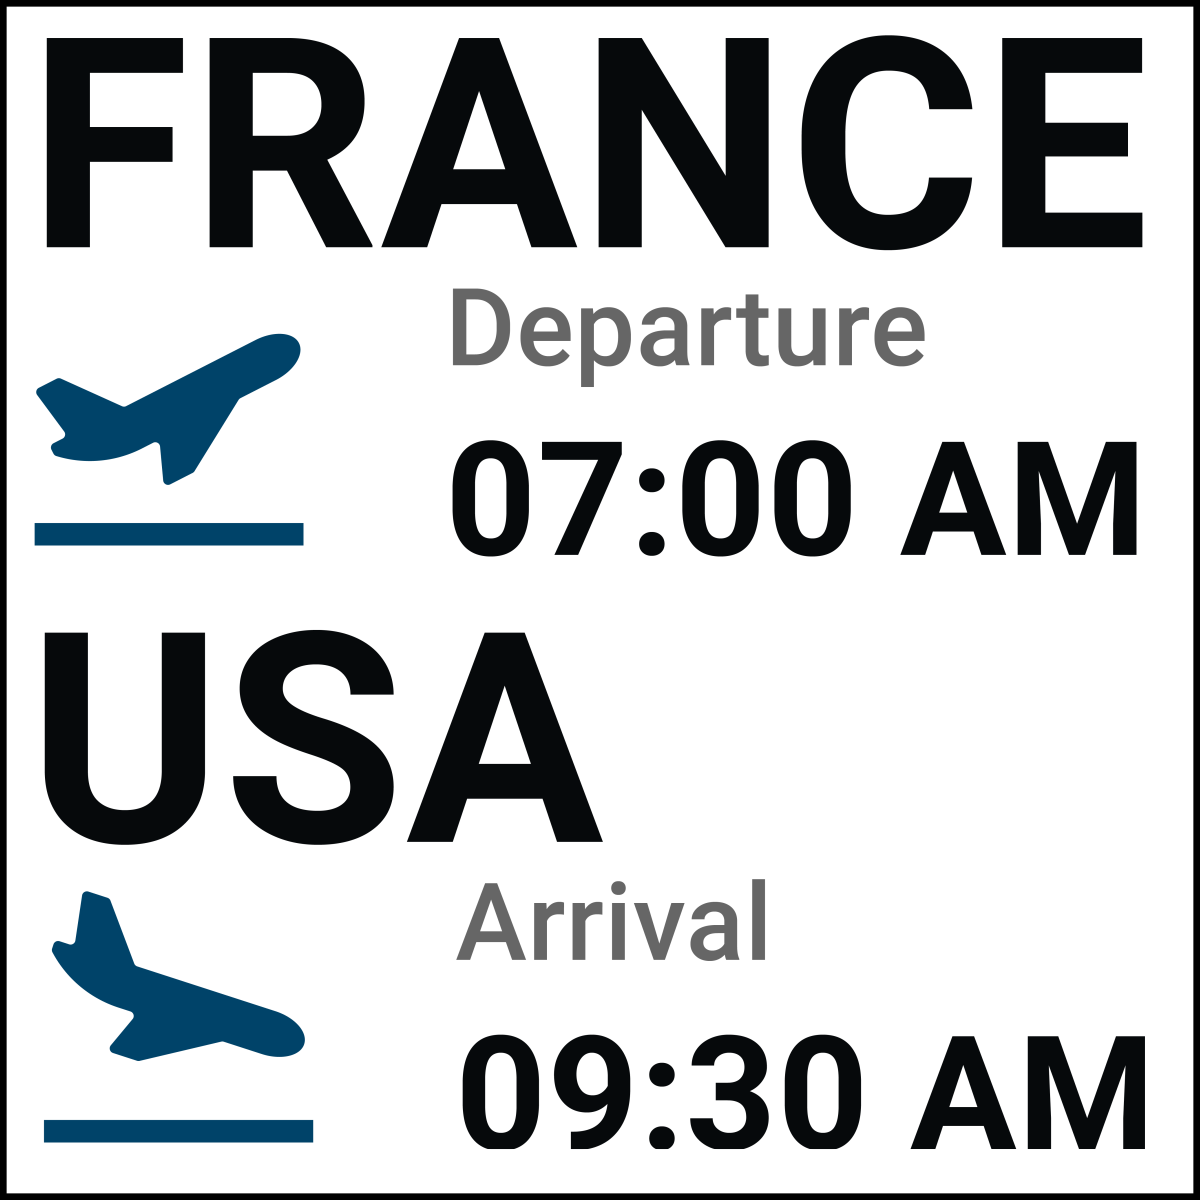
\includegraphics[width=0.5\textwidth]{Images/chapter_25/section_5890216939487232/5045247647416320.png}
\end{minipage}

% \vspace{-1.0\baselineskip}
\noindent
\begin{minipage}[t]{0.48\textwidth}\vspace{0pt}
\textbf{R5:} The admin should be able to add new flights and update or cancel scheduled flights.
\\
\textbf{R6:} An airline should be able to own multiple aircraft, and the admin should be able to add these aircraft to the system.
\\
\textbf{R7:} An airline should be able to operate its flights from different airports.
\\
\textbf{R8:} The admin should be able to effectively assign pilots and crew members to flights.
\end{minipage}
\hfill
\begin{minipage}[t]{0.48\textwidth}\vspace{0pt}
\centering
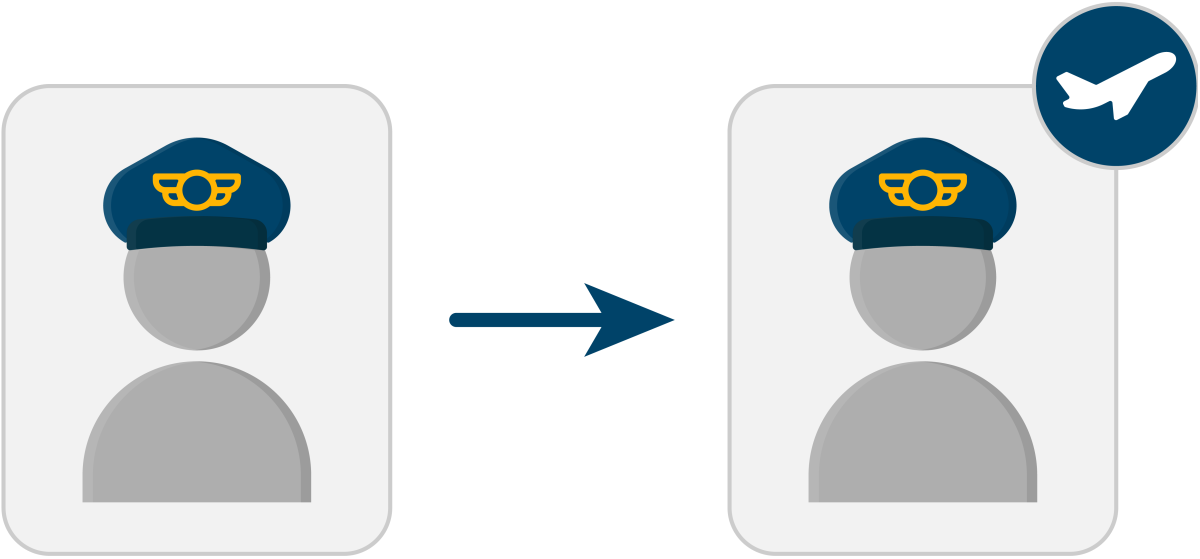
\includegraphics[width=0.5\textwidth]{Images/chapter_25/section_5890216939487232/6610553159286784.png}
\end{minipage}

% \vspace{-1.0\baselineskip}
\noindent
\begin{minipage}[t]{0.48\textwidth}\vspace{0pt}
\textbf{R9:} The customer should be able to make payments against their flight reservations.
\\
\textbf{R10:} The customer should be able to cancel their previous reservations.
\\
\textbf{R11:} The front desk officer should be able to reserve tickets, create itineraries, and make flight payments for the customer.
\\
\textbf{R12:} The flight crew should be able to view the schedule for their assigned flights.
\\
\textbf{R13:} The system should notify the customer whenever a reservation is made or canceled, or when there is an update regarding their flight.
\end{minipage}
\hfill
\begin{minipage}[t]{0.48\textwidth}\vspace{0pt}
\centering
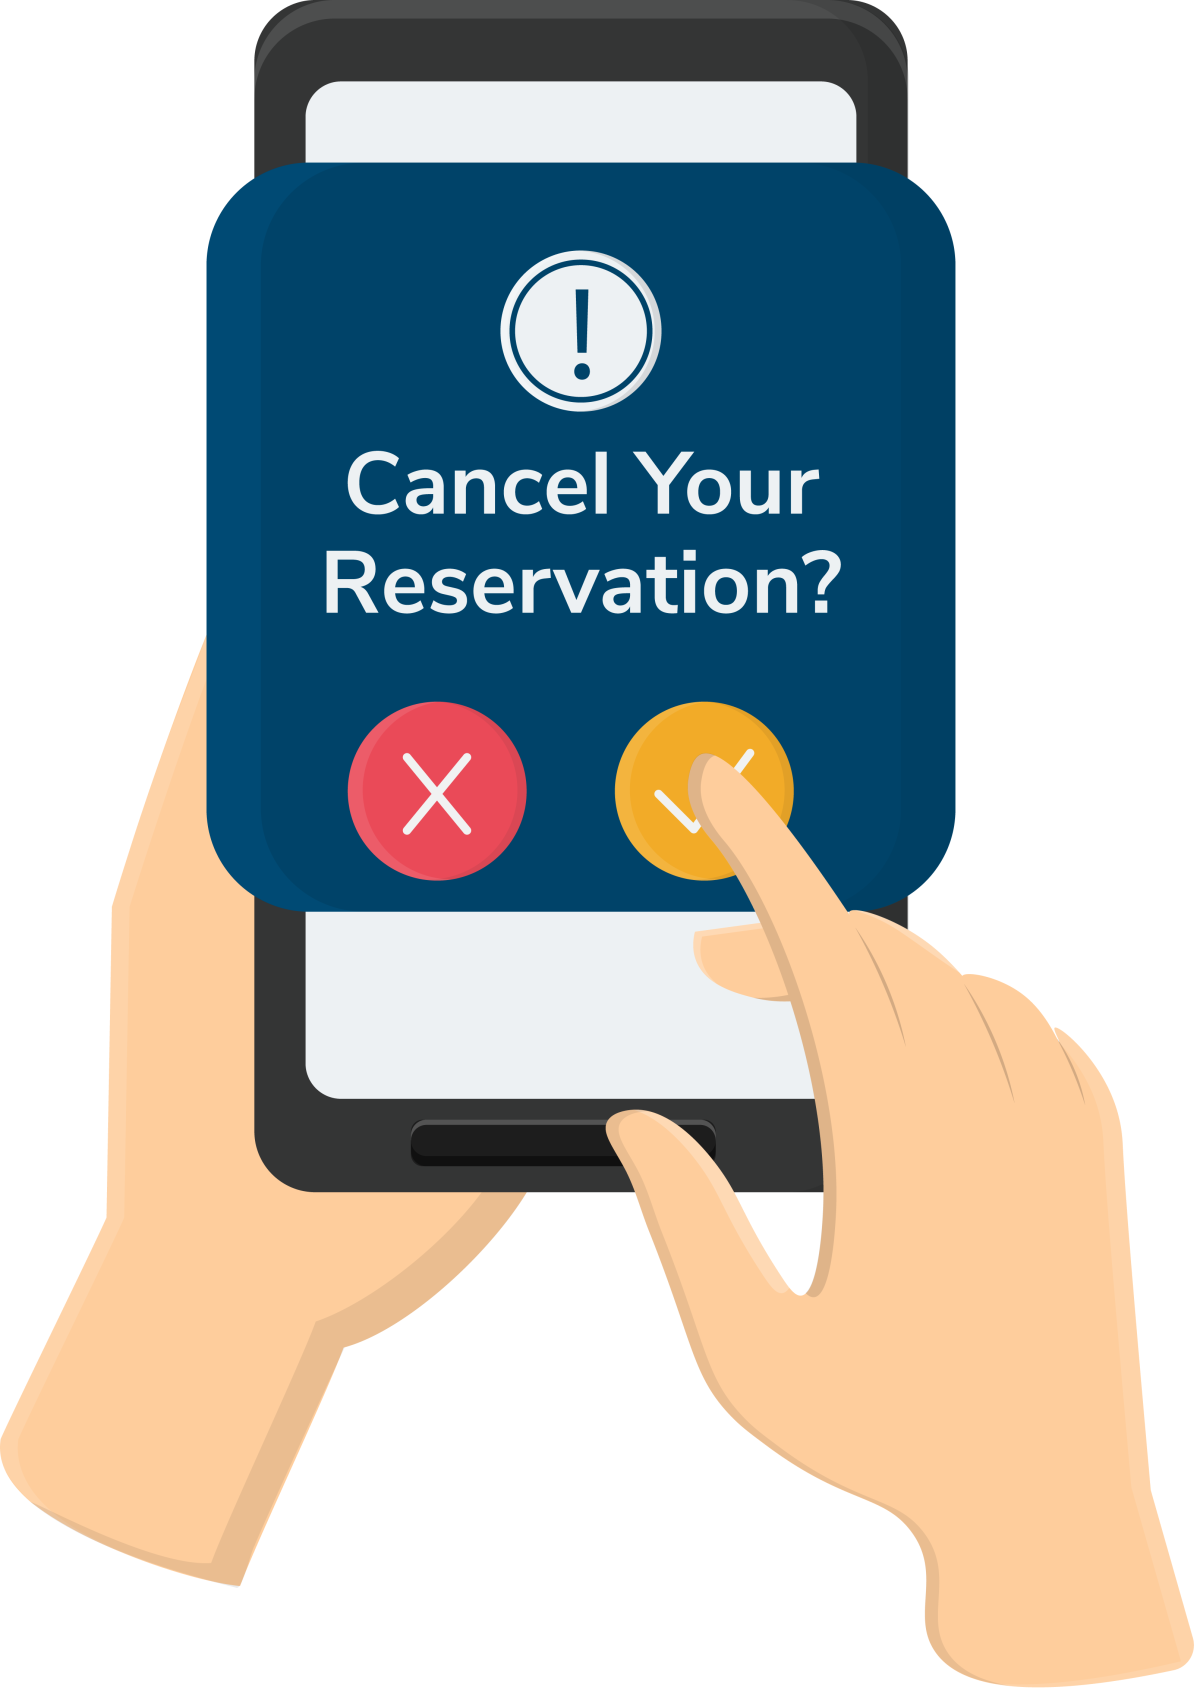
\includegraphics[width=0.5\textwidth]{Images/chapter_25/section_5890216939487232/5042039323623424.png}
\end{minipage}

We've identified our requirements for the problem. In the next lesson, we will define different use cases of the airline management system.

% End of section content